% This file was created by matplotlib2tikz v0.6.15.
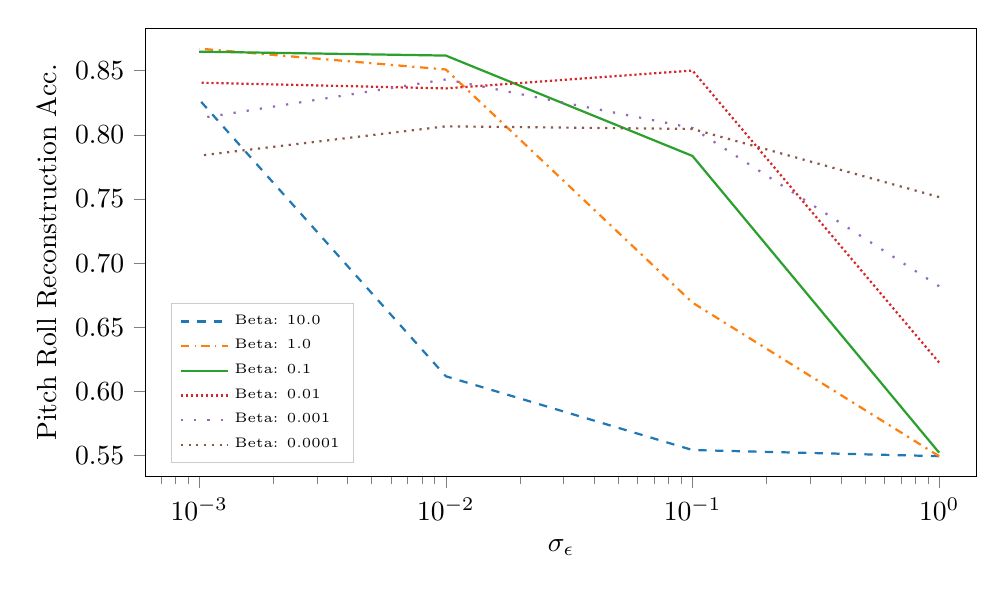
\begin{tikzpicture}

\definecolor{color0}{rgb}{0.12156862745098,0.466666666666667,0.705882352941177}
\definecolor{color3}{rgb}{0.83921568627451,0.152941176470588,0.156862745098039}
\definecolor{color4}{rgb}{0.580392156862745,0.403921568627451,0.741176470588235}
\definecolor{color1}{rgb}{1,0.498039215686275,0.0549019607843137}
\definecolor{color2}{rgb}{0.172549019607843,0.627450980392157,0.172549019607843}
\definecolor{color5}{rgb}{0.549019607843137,0.337254901960784,0.294117647058824}

\begin{axis}[
%title={Max pitch reconstruction accuracy on test set},
xlabel={$\sigma_{\epsilon}$},
ylabel={Pitch Roll Reconstruction Acc.},
xmin=0.000607945784384139, xmax=1.41253754462275,
ymin=0.533663075897538, ymax=0.883058500064946,
height = 0.60\columnwidth,
width= 1.0\columnwidth,
xmode=log,
xtick={1e-05,0.0001,0.001,0.01,0.1,1,10,100},
xticklabels={$10^{-5}$,$10^{-4}$,$10^{-3}$,$10^{-2}$,$10^{-1}$,$10^{0}$,$10^{1}$,$10^{2}$},
ytick={0.5,0.55,0.6,0.65,0.7,0.75,0.8,0.85,0.9},
yticklabels={0.50,0.55,0.60,0.65,0.70,0.75,0.80,0.85,0.90},
tick align=outside,
tick pos=left,
x grid style={lightgray!92.02614379084967!black},
y grid style={lightgray!92.02614379084967!black},
legend cell align={left},
legend style={at={(0.03,0.03)}, anchor=south west, draw=white!80.0!black, font=\tiny, fill=none},
legend entries={{Beta: 10.0},{Beta: 1.0},{Beta: 0.1},{Beta: 0.01},{Beta: 0.001},{Beta: 0.0001}}
]
\addlegendimage{no markers, color0, dashed, thick}
\addlegendimage{no markers, color1,dashdotted, thick}
\addlegendimage{no markers, color2, thick}
\addlegendimage{no markers, color3, densely dotted, thick}
\addlegendimage{no markers, color4, loosely dotted, thick}
\addlegendimage{no markers, color5, dotted, thick}
\addplot [thick, color0, dashed]
table {%
1 0.549544686086965
0.1 0.554330248782514
0.01 0.611815060288938
0.001 0.827379658124794
};
\addplot [thick, color1, dashdotted]
table {%
1 0.549546092925563
0.1 0.669208481396159
0.01 0.850884461081067
0.001 0.867176889875518
};
\addplot [thick, color2]
table {%
1 0.55226648847399
0.1 0.783504715863829
0.01 0.861739100979037
0.001 0.864804829706785
};
\addplot [thick, color3,densely dotted]
table {%
1 0.622474812590917
0.1 0.850092921828988
0.01 0.83615603173379
0.001 0.840622539775086
};
\addplot [thick, color4, loosely dotted]
table {%
1 0.681979140055659
0.1 0.805310639710232
0.01 0.843174112788324
0.001 0.812846656528773
};
\addplot [thick, color5, dotted]
table {%
1 0.751471941225575
0.1 0.804555928977962
0.01 0.806602212593752
0.001 0.783772318700316
};
% \path [draw=black, fill opacity=0] (axis cs:0,0.533663075897538)
% --(axis cs:0,0.883058500064946);

% \path [draw=black, fill opacity=0] (axis cs:1,0.533663075897538)
% --(axis cs:1,0.883058500064946);

% \path [draw=black, fill opacity=0] (axis cs:0.000707945784384139,0)
% --(axis cs:1.41253754462275,0);

% \path [draw=black, fill opacity=0] (axis cs:0.000707945784384139,1)
% --(axis cs:1.41253754462275,1);

% \draw[] (axis cs:0.1,0.554330248782514) -- (axis cs:0.1,0.554330248782514);
% \node at (axis cs:0.1,0.554330248782514)[
%   scale=0.35,
%   anchor=base west,
%   text=black,
%   rotate=0.0
% ]{ 0.1772108901719074};
% \draw[] (axis cs:0.01,0.611815060288938) -- (axis cs:0.01,0.611815060288938);
% \node at (axis cs:0.01,0.611815060288938)[
%   scale=0.35,
%   anchor=base west,
%   text=black,
%   rotate=0.0
% ]{ 0.01114844633403056};
% \draw[] (axis cs:0.1,0.669208481396159) -- (axis cs:0.1,0.669208481396159);
% \node at (axis cs:0.1,0.669208481396159)[
%   scale=0.35,
%   anchor=base west,
%   text=black,
%   rotate=0.0
% ]{ 0.3911486546426436};
% \draw[] (axis cs:0.01,0.850884461081067) -- (axis cs:0.01,0.850884461081067);
% \node at (axis cs:0.01,0.850884461081067)[
%   scale=0.35,
%   anchor=base west,
%   text=black,
%   rotate=0.0
% ]{ 0.4891881473937402};
% \draw[] (axis cs:0.1,0.783504715863829) -- (axis cs:0.1,0.783504715863829);
% \node at (axis cs:0.1,0.783504715863829)[
%   scale=0.35,
%   anchor=base west,
%   text=black,
%   rotate=0.0
% ]{ 0.5952689852109977};
% \draw[] (axis cs:0.01,0.861739100979037) -- (axis cs:0.01,0.861739100979037);
% \node at (axis cs:0.01,0.861739100979037)[
%   scale=0.35,
%   anchor=base west,
%   text=black,
%   rotate=0.0
% ]{ 0.46272865103907806};
% \draw[] (axis cs:0.1,0.850092921828988) -- (axis cs:0.1,0.850092921828988);
% \node at (axis cs:0.1,0.850092921828988)[
%   scale=0.35,
%   anchor=base west,
%   text=black,
%   rotate=0.0
% ]{ 0.48928990101099834};
% \draw[] (axis cs:0.01,0.83615603173379) -- (axis cs:0.01,0.83615603173379);
% \node at (axis cs:0.01,0.83615603173379)[
%   scale=0.35,
%   anchor=base west,
%   text=black,
%   rotate=0.0
% ]{ 0.3791896834076692};
% \draw[] (axis cs:0.1,0.805310639710232) -- (axis cs:0.1,0.805310639710232);
% \node at (axis cs:0.1,0.805310639710232)[
%   scale=0.35,
%   anchor=base west,
%   text=black,
%   rotate=0.0
% ]{ 0.4112820375159996};
% \draw[] (axis cs:0.01,0.843174112788324) -- (axis cs:0.01,0.843174112788324);
% \node at (axis cs:0.01,0.843174112788324)[
%   scale=0.35,
%   anchor=base west,
%   text=black,
%   rotate=0.0
% ]{ 0.44158474779355006};
% \draw[] (axis cs:0.1,0.804555928977962) -- (axis cs:0.1,0.804555928977962);
% \node at (axis cs:0.1,0.804555928977962)[
%   scale=0.35,
%   anchor=base west,
%   text=black,
%   rotate=0.0
% ]{ 0.3888835104154009};
% \draw[] (axis cs:0.01,0.806602212593752) -- (axis cs:0.01,0.806602212593752);
% \node at (axis cs:0.01,0.806602212593752)[
%   scale=0.35,
%   anchor=base west,
%   text=black,
%   rotate=0.0
% ]{ 0.42906802229475877};
\end{axis}

\end{tikzpicture}